% \iffalse
\let\negmedspace\undefined
\let\negthickspace\undefined
\documentclass[journal,12pt,twocolumn]{IEEEtran}
\usepackage{cite}
\usepackage{amsmath,amssymb,amsfonts,amsthm}
\usepackage{algorithmic}
\usepackage{graphicx}
\usepackage{textcomp}
\usepackage{xcolor}
\usepackage{txfonts}
\usepackage{listings}
\usepackage{enumitem}
\usepackage{mathtools}
\usepackage{gensymb}
\usepackage{comment}
\usepackage[breaklinks=true]{hyperref}
\usepackage{tkz-euclide} 
\usepackage{listings}
\usepackage{gvv}                                        
\def\inputGnumericTable{}                                 
\usepackage[latin1]{inputenc}                                
\usepackage{color}                                            
\usepackage{array}                                            
\usepackage{longtable}                                       
\usepackage{calc}                                             
\usepackage{multirow}                                         
\usepackage{hhline}                                           
\usepackage{ifthen}                                           
\usepackage{lscape}
\newtheorem{theorem}{Theorem}[section]
\newtheorem{problem}{Problem}
\newtheorem{proposition}{Proposition}[section]
\newtheorem{lemma}{Lemma}[section]
\newtheorem{corollary}[theorem]{Corollary}
\newtheorem{example}{Example}[section]
\newtheorem{definition}[problem]{Definition}
\newcommand{\BEQA}{\begin{eqnarray}}
\newcommand{\EEQA}{\end{eqnarray}}
\newcommand{\define}{\stackrel{\triangle}{=}}
\theoremstyle{remark}
\newtheorem{rem}{Remark}
\begin{document}

\bibliographystyle{IEEEtran}
\vspace{3cm}

\title{11.9.4.7}
\author{EE23BTECH11063 - Vemula Siddhartha
}
\maketitle
\newpage
\bigskip

\renewcommand{\thefigure}{\theenumi}
\renewcommand{\thetable}{\theenumi}
\textbf{Question}:\\
Find the sum to $n$ terms of the series:
\begin{align*}
    1^2+\brak{1^2+2^2}+\brak{1^2+2^2+3^2}+...
\end{align*}
\textbf{Solution:}
\begin{table}[h!]    
    \centering
    \begin{tabular}[12pt]{ |c| c|}
    \hline
    \textbf{Symbol} & \textbf{Description}\\ 
    \hline
    $ f\brak{x} $ & Function \\
    \hline 
    $ G\brak{f} $ & Fourier Transform of the function $ f\brak{x} $ \\
    \hline
    $ f^*\brak{x} $ & Complex Conjugate of $ f\brak{x} $ \\
    \hline
    $ G^*\brak{f} $ & Complex Conjugate of $ G\brak{f} $ \\
    \hline
    Im$ \brak{ G \brak{ f } }$ & Imaginary Part of $ G\brak{f} $ \\
    \hline
    \end{tabular}
    \caption{Variables Used}
    \label{tab10.5.3.9.1}
  \end{table}
\begin{align}
    y\brak{n}&=1^2+\brak{1^2+2^2}+\brak{1^2+2^2+3^2}+...\\
    x\brak{n}&=\sum_{k=0}^{n}\brak{k+1}^2u\brak{k}\\
    x\brak{n}&=\brak{\brak{n+1}^2u\brak{n}}*u\brak{n}\\
    X\brak{z}&=Z\cbrak{\brak{n+1}^2u\brak{n}}U\brak{z}\\
    &=\brak{\frac{1+z^{-1}}{\brak{1-z^{-1}}^3}}\brak{\frac{1}{1-z^{-1}}}\\
    X\brak{z}&=\frac{1+z^{-1}}{\brak{1-z^{-1}}^4}\\
    y\brak{n}&=x\brak{n}*u\brak{n}\\
    Y\brak{z}&=X\brak{z}U\brak{z}\\
    &=\brak{\frac{1+z^{-1}}{\brak{1-z^{-1}}^4}}\brak{\frac{1}{1-z^{-1}}}\\
    &=\frac{z^4\brak{z+1}}{\brak{z-1}^5}
\end{align}
Taking the Inverse $Z$ transform, from Contour Integration,
\begin{align}
    y\brak{n}&=\frac{1}{2\pi j}\oint_C\frac{z^4\brak{z+1}}{\brak{z-1}^5}\:z^{n-1}dz\\
    &=\frac{1}{\brak{k-1}!} \lim_{z\to c}\frac{d^{k-1}}{dz^{k-1}}\brak{\brak{z-c}^kf\brak{z}}\\
    &=\frac{1}{4!}\lim_{z\to1}\frac{d^4}{dz^4}\brak{\brak{z-1}^5\frac{z^4\brak{z+1}}{\brak{z-1}^5}\:z^{n-1}}\\
    &=\frac{1}{24}\lim_{z\to1}\frac{d^4}{dz^4}\brak{z^{n+4}+z^{n+3}}\\
    \implies y\brak{n}&=\frac{\brak{n+1}\brak{n+2}^2\brak{n+3}}{12}\;u\brak{n}
\end{align}
\begin{figure}[h!]
    \centering
    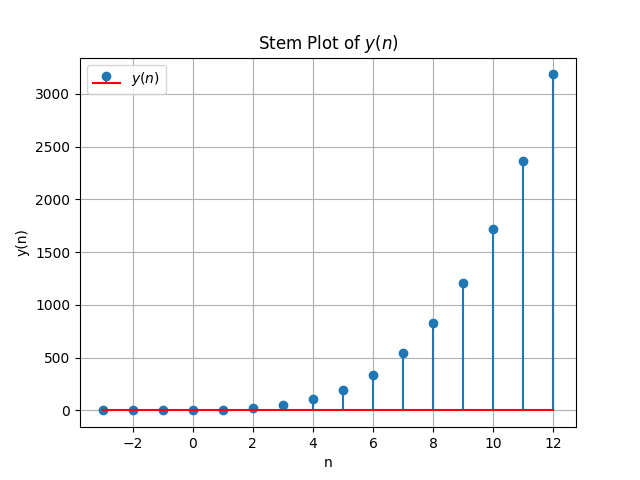
\includegraphics[width=1\linewidth]{figs/Figure_1.png}
    \caption{Stem Plot of y\brak{n}}
\end{figure}
\end{document}